%%%%%%%%%%%%%%%%%%%
%                                                        %
% SHPECK - SPECIATION MODEL  %
%                                                        %
%%%%%%%%%%%%%%%%%%%


\chapter{\emph{SHPECK} - Speciation Model}
\label{chapter:SHPECK}

\emph{SHPECK} is a equation-based simulator, there is a governing theory that can guide the construction of mathematical models based on a set of equations. The “equation-based” term refers to simulations based on the kinds of global equations we associate with physical theories - many of these theories present in the foundation concepts of \emph{SHPECK} originally from the \emph{Phase Rule}. Phase rule allows us to predict the number of stable phases that may exist in equilibrium for a particular system and is describe fully in \cite{Garrels:65} and is the base principle used in chemical speciation.

As a computer simulation software, \emph{SHPECK} represents the entire process. This process includes choosing a model; finding a way of implementing that model in a form that a computer can run; calculating the output of the algorithm; visualizing and studying the resultant data.

This chapter will guide through all the aspects of the development of \emph{SHPECK} - a geochemical speciation modelling software. 

\section{Specification}
\emph{SHPECK} is a geochemical speciation modelling software responsible for calculating the distribution of dissolved species between free ions and aqueous complexes and also saturation indexes for different minerals. 

\section{Architecture}
The architecture of a software is responsible for assuring that all the internal and external stakeholders' concerns are preserved, addressed and satisfied. To not develop something that will not need restructuration and code refactoring later, it is necessary to see the big picture of the whole \emph{SHPECK}'s project. This will drive and be present during the entire development, starting with the technical decisions until the satisfaction of the final user.

Figure ~\ref{fig:shpeck-architecture} brings the software architecture of \emph{SHPECK}, which is modelled following the popular concept of \emph{Model-View-Controller} (MVC) \cite{Gamma:94}. \emph{MVC} is an architectural pattern that divides the software into three interconnected parts:
\begin{itemize}
\item Model: It is an object representing data or even activity. For example, the algorithm and math behind calculating the activity coefficient by Debye-Huckels' formula.
\item View: It is some form of visualization of the state of the model. For example, which are the solutes that the user wants to add into the simulation?
\item Controller: It offers facilities to change the state of the model. For example, define which algorithm for calculating the activity coefficient according to the user's choice or the value of the ionic strength (if the user did not specify which one to use).
\end{itemize}

\begin{figure}[ht!]
\centering
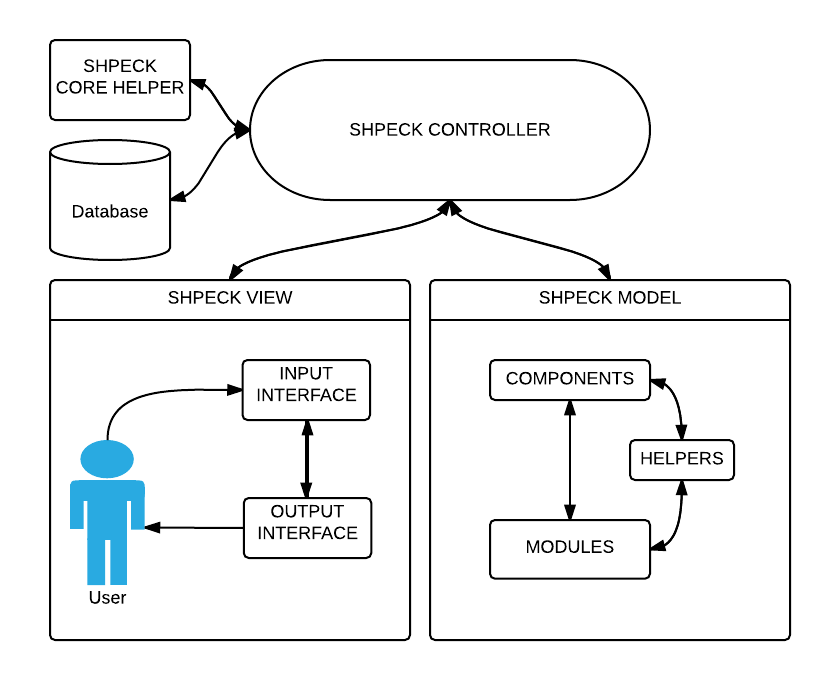
\includegraphics[width=100mm]{figures/shpeck-architecture.png}
\caption{Architecture of the \emph{SHPECK} software}
\label{fig:shpeck-architecture}
\end{figure}

\subsection{Technical Specification}
\emph{SHPECK} is a software developed using C++, which is a general-purpose programming language. C++ has a bias towards system programming that supports efficient low-level computation, data abstraction, object-oriented programming, and generic programming \cite{Dale:04} \cite{Stroustrup:97}. It provides powerful and flexible mechanisms for abstraction; that is, language constructs that allow the programmer to introduce and use new types of objects that match the concepts of an application needed. Thus, C++ supports styles of programming that rely on relatively direct manipulation of hardware resources to deliver a high degree of efficiency. It can also address higher-level styles of programming that rely on user-defined types to provide a model of computation that is closer to human's view of the task being performed by a computer. Application libraries often support these higher level styles of programming. While developing Shpeck, two supporter tools were adopted:
\begin{itemize}
\item \emph{Qt} : It is a cross-platform application and UI framework for developers using C++  \cite{Qt:14}. \emph{Qt} turns the development fast and easy, with lots of inbuilt library classes it provides a comprehensive range of functionality which also turns the debugging and testing way more productive and effective.
\item \emph{Armadillo} : It Is a C++ linear algebra library that provides classes for vectors, matrices, cubes and a whole set of functions to operate on the classes \cite{arma:14}. With a syntax similar to Matlab and an up-to-date support with upgrades and new releases almost every month.
\end{itemize}
Important to mention that the system is being developed using \emph{MAC} but the whole development process always took into account the goal to develop a multi-platform software to be distributed either in \emph{Windows, UNIX} and \emph{MAC}.

\section{Governing equations}
%These chemical equations are a mathematical model that drives all the methods that are executed in \emph{SHPECK}, its behavior defines all the steps and in which order they are presented. This set of equations models a real-world system and is named \emph{computer simulation model}.

\emph{SHPECK} uses the thermodynamic equilibrium reaction as equations for the calculation of multiphase systems in equilibrium, the details of these reactions are discussed in details in chapter ~\ref{chapter:basic}. A set of mass-action equations (as in equation ~\ref{eq:massaction}) compose the system; The number of species and compounds that coexist in the system define the number of equations. These equations model the geochemical speciation closed system and take into account all the chemical properties.

Aside with the mass-action equations we must have other constraints to solve the equilibrium state of the system. In \emph{SHPECK}, we use the concentration of the species (other possible constraints are the solute activity, the number of moles, total volume, etc.) to deal with the equilibrium state of the system.
This configuration generates a system where there are \emph{U} unknowns, {M} mass-action equations and \emph{E} equilibrium constraints. 
\begin{equation}\label{equilibrium_reaction}
U = E + M
\end{equation}
The unknowns values represents the number of moles of each specie in the system.

\section{Numerical Method}
In order to solve the system composed of the equilibrium state of the mass-action equations and the equilibrium constraints, \emph{SHPECK} uses a numerical methodology that computes simultaneously and find the value of the unknowns.


The numerical method applied a modification of the \emph{Newton's method} (also known as Newton-Raphson method), which is a method for finding successively better approximations to the roots of a set of equations. It works with a derivative approach to the equations, which optimizes the time consumed to find the roots and makes the representation of the system easier.

\emph{SHPECK} uses the \emph{Gauss-Newton}'s method to solve a nonlinear system of equations which results in finding the roots of continuously differentiable equations. 

The \emph{Gauss-Newton}'s method is applied in order to achieve the best approximation possible to the solution that is being sought. It since it is an iterative algorithm where each step consists in minimizing the first-order approximation of the solution. \emph{Gauss-Newton}'s method is a modification of \emph{Newton}'s method (also known as \emph{Newton-Raphson}'s method) for finding a minimum of a function. Its difference from regular \emph{Newton}'s method is that second derivatives are not required. \emph{Gauss-Newton}'s method is used to solve a system of coupled nonlinear equations. The first-order approximation of the function starts with an initial guess for the minimum values, the method proceeds by the iterations as shown in equations ~\ref{eq:gaussNewtonMethodEq1} and ~\ref{eq:gaussNewtonMethodEq2}.

\begin{equation}
\label{eq:gaussNewtonMethodEq1}
F(x+1) = F(x) - J^{-1} * R
\end{equation}

or 

\begin{equation}
\label{eq:gaussNewtonMethodEq2}
F(x+1) = F(x) - \frac{F(x)}{F'(x)}
\end{equation}

Where $F$ is function's result for the applied $x$, $J^{-1}$ is the inverse of the Jacobian matrix, and $R$ is the residual matrix \cite{Isaacson:66}.

The $R$ residual vector is defined as a vector containing the resulting values for each equation.

\begin{equation}
\label{eq:residualVector}
R = \begin{pmatrix}
 F(x_1) \\
 \vdots \\
 F(x_m)
 \end{pmatrix}
\end{equation}

Where $m$ is the number of unknowns (or mass-action equations plus equilibrium constraints).


The algorithm consists of iteratively calculating new approximations for the unknown values, through the matrix equation:

\begin{equation}
\label{eq:iterativelyAlgorithm}
[J]^{-1}_{iteration}* \alpha [U]_{iteration+1} = [R]_{iteration}
\end{equation}

Where $J$ is the Jacobian Matrix; $ \alpha [U]_{iteration+1} $ is the unknown composition at the next iteration; iteration is the iteration number and $R$ is the residual matrix. With this, is possible to state the $[U]_{iteration+1}$ value with:

\begin{equation}
\label{eq:CompositionCalculation}
[U]_{iteration+1} = [U]_{iteration} + \alpha [U]_{iteration+1}
\end{equation}


The initial guess of the solutions is an approximation that the user provides to the \emph{Gauss-Newton}'s method. This method needs a \emph{seed} to start the calculations (usually this guess is used for $F(0)$). 
If the guess is close to the real root value than the number of iterations necessary to obtain the solution will be small. If the guess is something completely nonsense, and far from the real solution, more iterations are going to be needed to find the correct solution.

The \emph{Jacobian Matrix} receives the equations and generates a model that does it automatically The \emph{Jacobian Matrix} is the matrix of all first-order partial derivatives of the equation and it is defined as

\begin{equation}
\label{eq:JacobianDefinition}
J_{mn} = \frac{\partial y^m}{\partial x^n}
\end{equation}

where the $y^i$'s are a new coordinate system defined in terms of the original coordinate system, the $x^i$'s. In differential equation theory, the Jacobian matrix plays a key role in defining the stability of solutions.

Specifically, \emph{SHPECK}'s equations can be described as: $F_1(x_1,..., x_n)$,...,$F_m(x_1,...,x_n)$. The partial derivatives of all these equations with respect to the variables $x_1,...,x_n$ can be organized in a m-by-n matrix, the Jacobian matrix, as bellow:

\begin{equation} 
J =
 \begin{pmatrix}
  \frac{\partial F_1}{\partial x_1} & \cdots & \frac{\partial F_1}{\partial x_n} \\
  \vdots  & \ddots & \vdots  \\
  \frac{\partial F_m}{\partial x_1} & \cdots &   \frac{\partial F_m}{\partial x_n}
 \end{pmatrix}
\end{equation}

In our case, $m = n$ and the \emph{jacobian matrix} is a square matrix and is generated once. With all the equations selected and organized, the derivatives of each reaction towards each variable are calculated and the \emph{jacobian matrix} is modeled and stored. 

Important to realize that the main complication with using a the \emph{Gauss-Newton}'s method to solve a system of nonlinear equations is defining all the functions included in the \emph{Jacobian Matrix}. As the number of equations and unknowns increases (n), so does the number of elements in the \emph{Jacobian} ($n^2$).

\section{Algorithm}

\emph{SHPECK}'s algorithm takes as its input a specification of the system's state. For example, the values for the concentrations of the species in the solution, the temperature of the system, the method to calculate activity coefficient, etc. It then calculates the system's state by executing all the processes in the necessary order that the model was conceptualized. 
Figure ~\ref{fig:Shpeck-algo} presents the high-level algorithm in details; is important to understand that each of the boxes in this algorithm represents a set of instructions, calculations and conditional clauses. Due to this work's scope we only specify the algorithm inside the box called "Newton's Method Solver", understanding how the governing equations controls the numerical methods is a fundamental piece. Newton's Method Solver internal algorithm is presented in figure ~\ref{fig:Shpeck-algo-newton}. 
\begin{figure}[ht!]
\centering
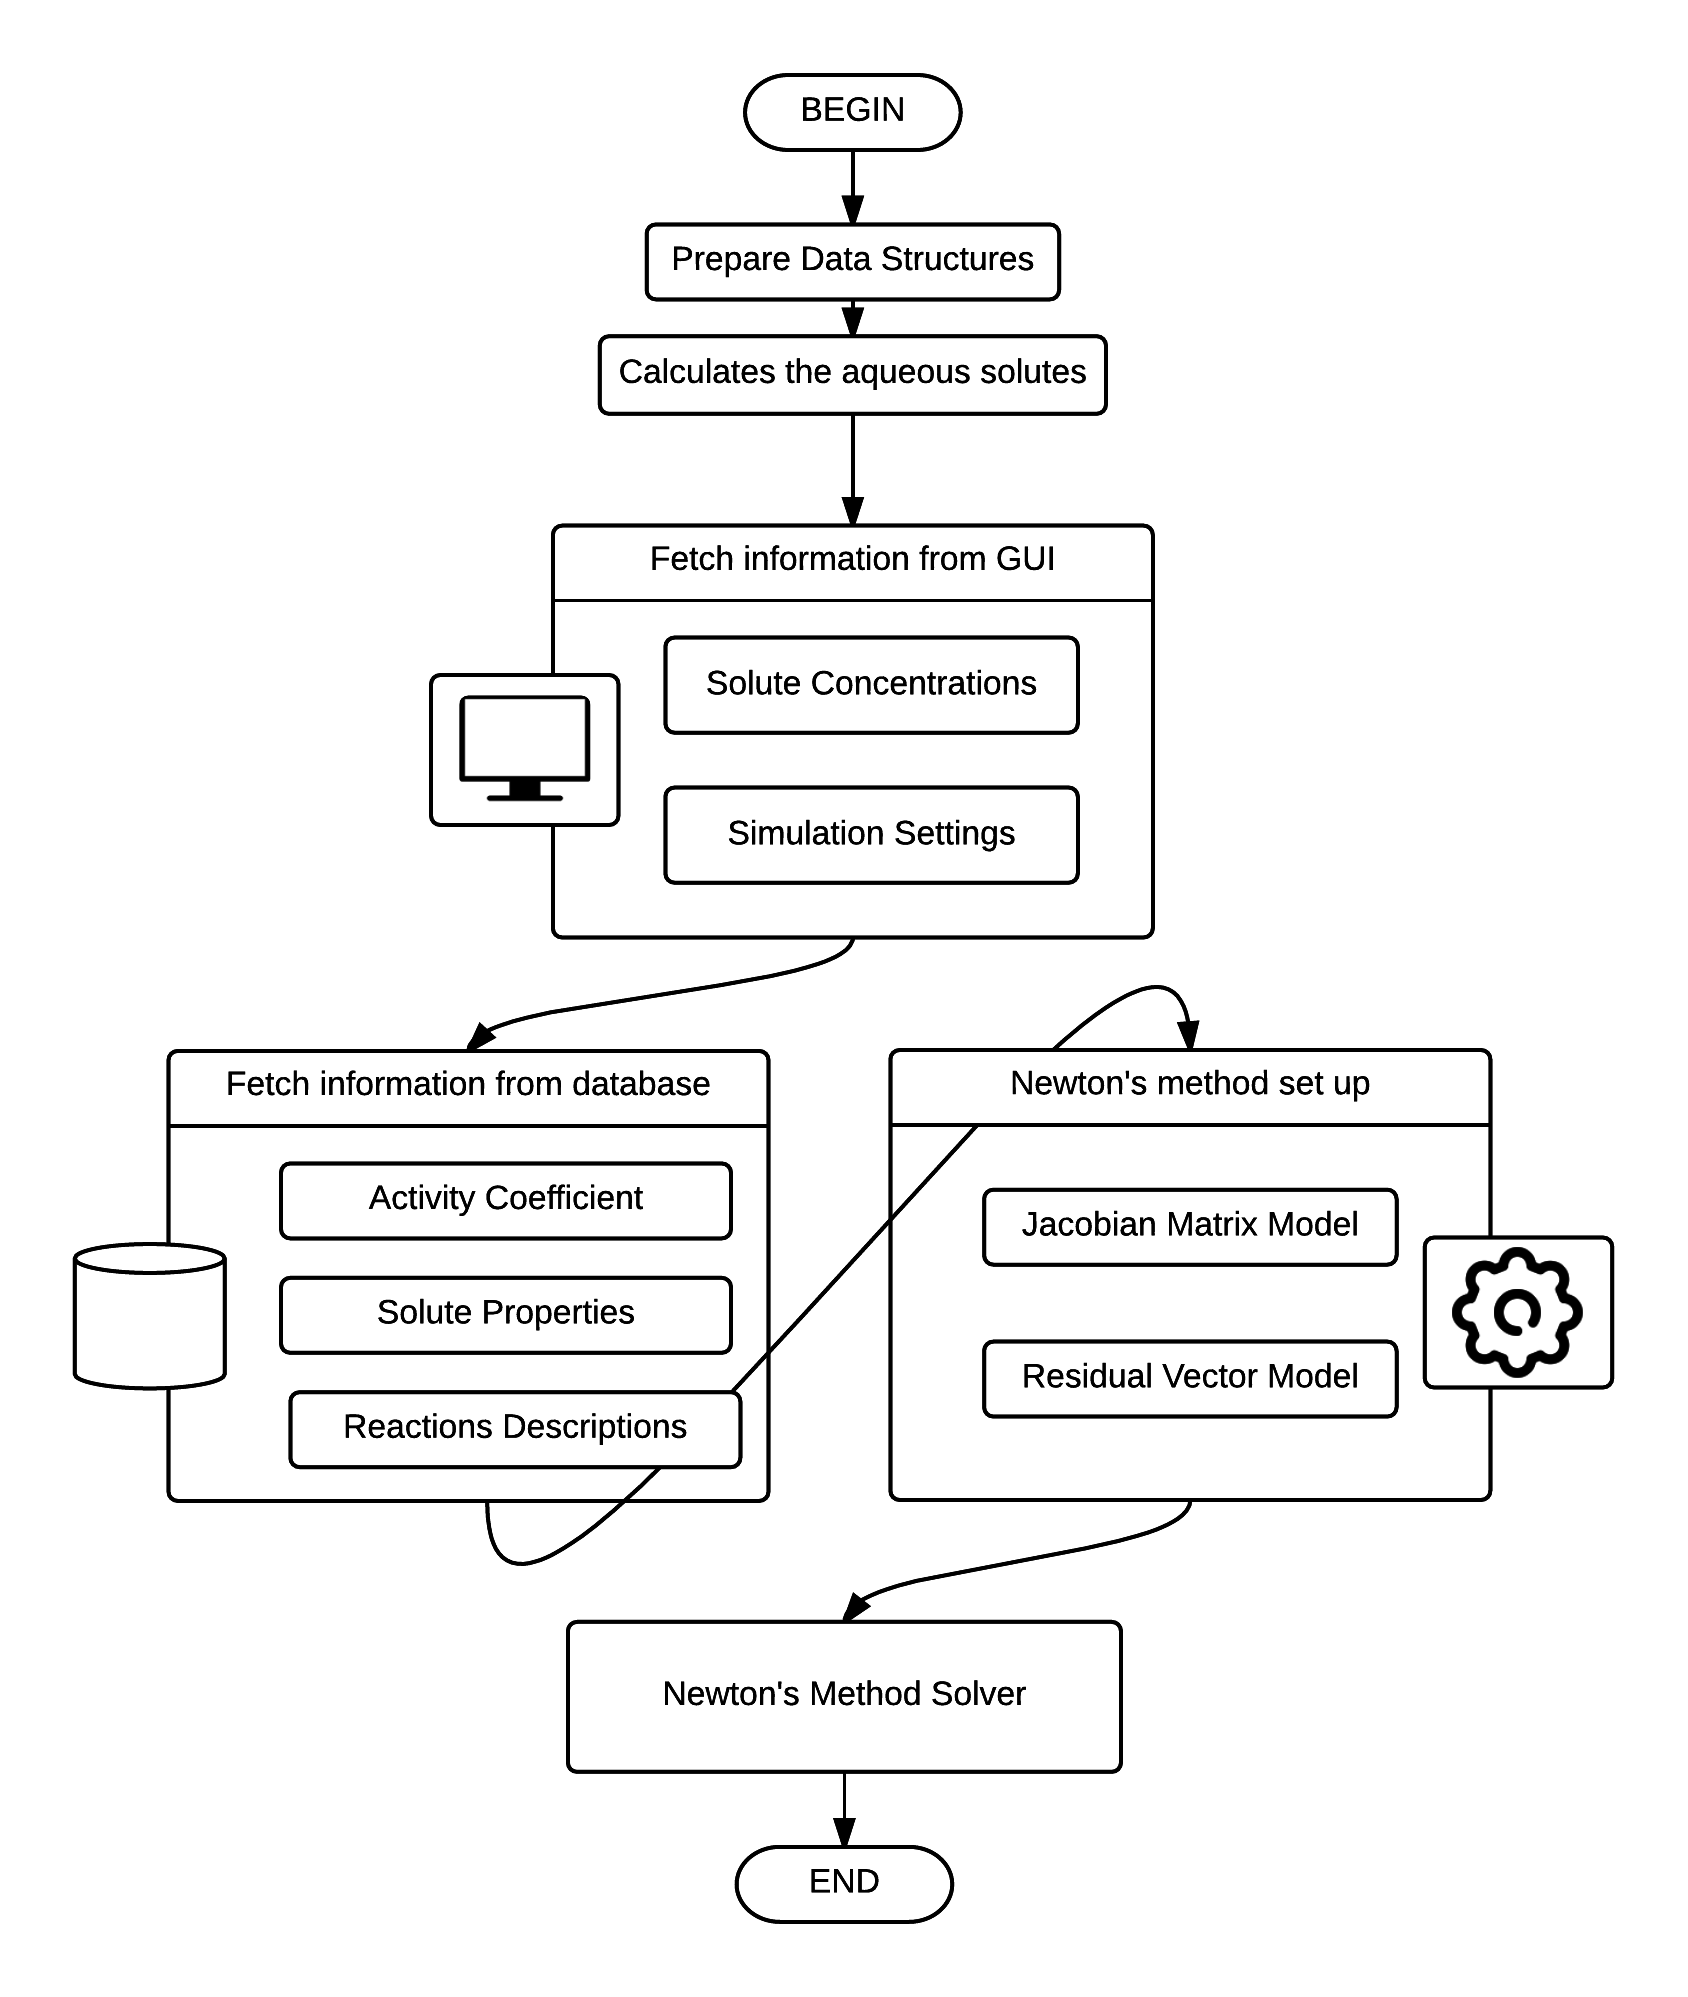
\includegraphics[width=100mm]{figures/Shpeck_algo3.png}
\caption{High-level algorithm of \emph{SHPECK}}
\label{fig:Shpeck-algo}
\end{figure}
\begin{figure}[ht!]
\centering
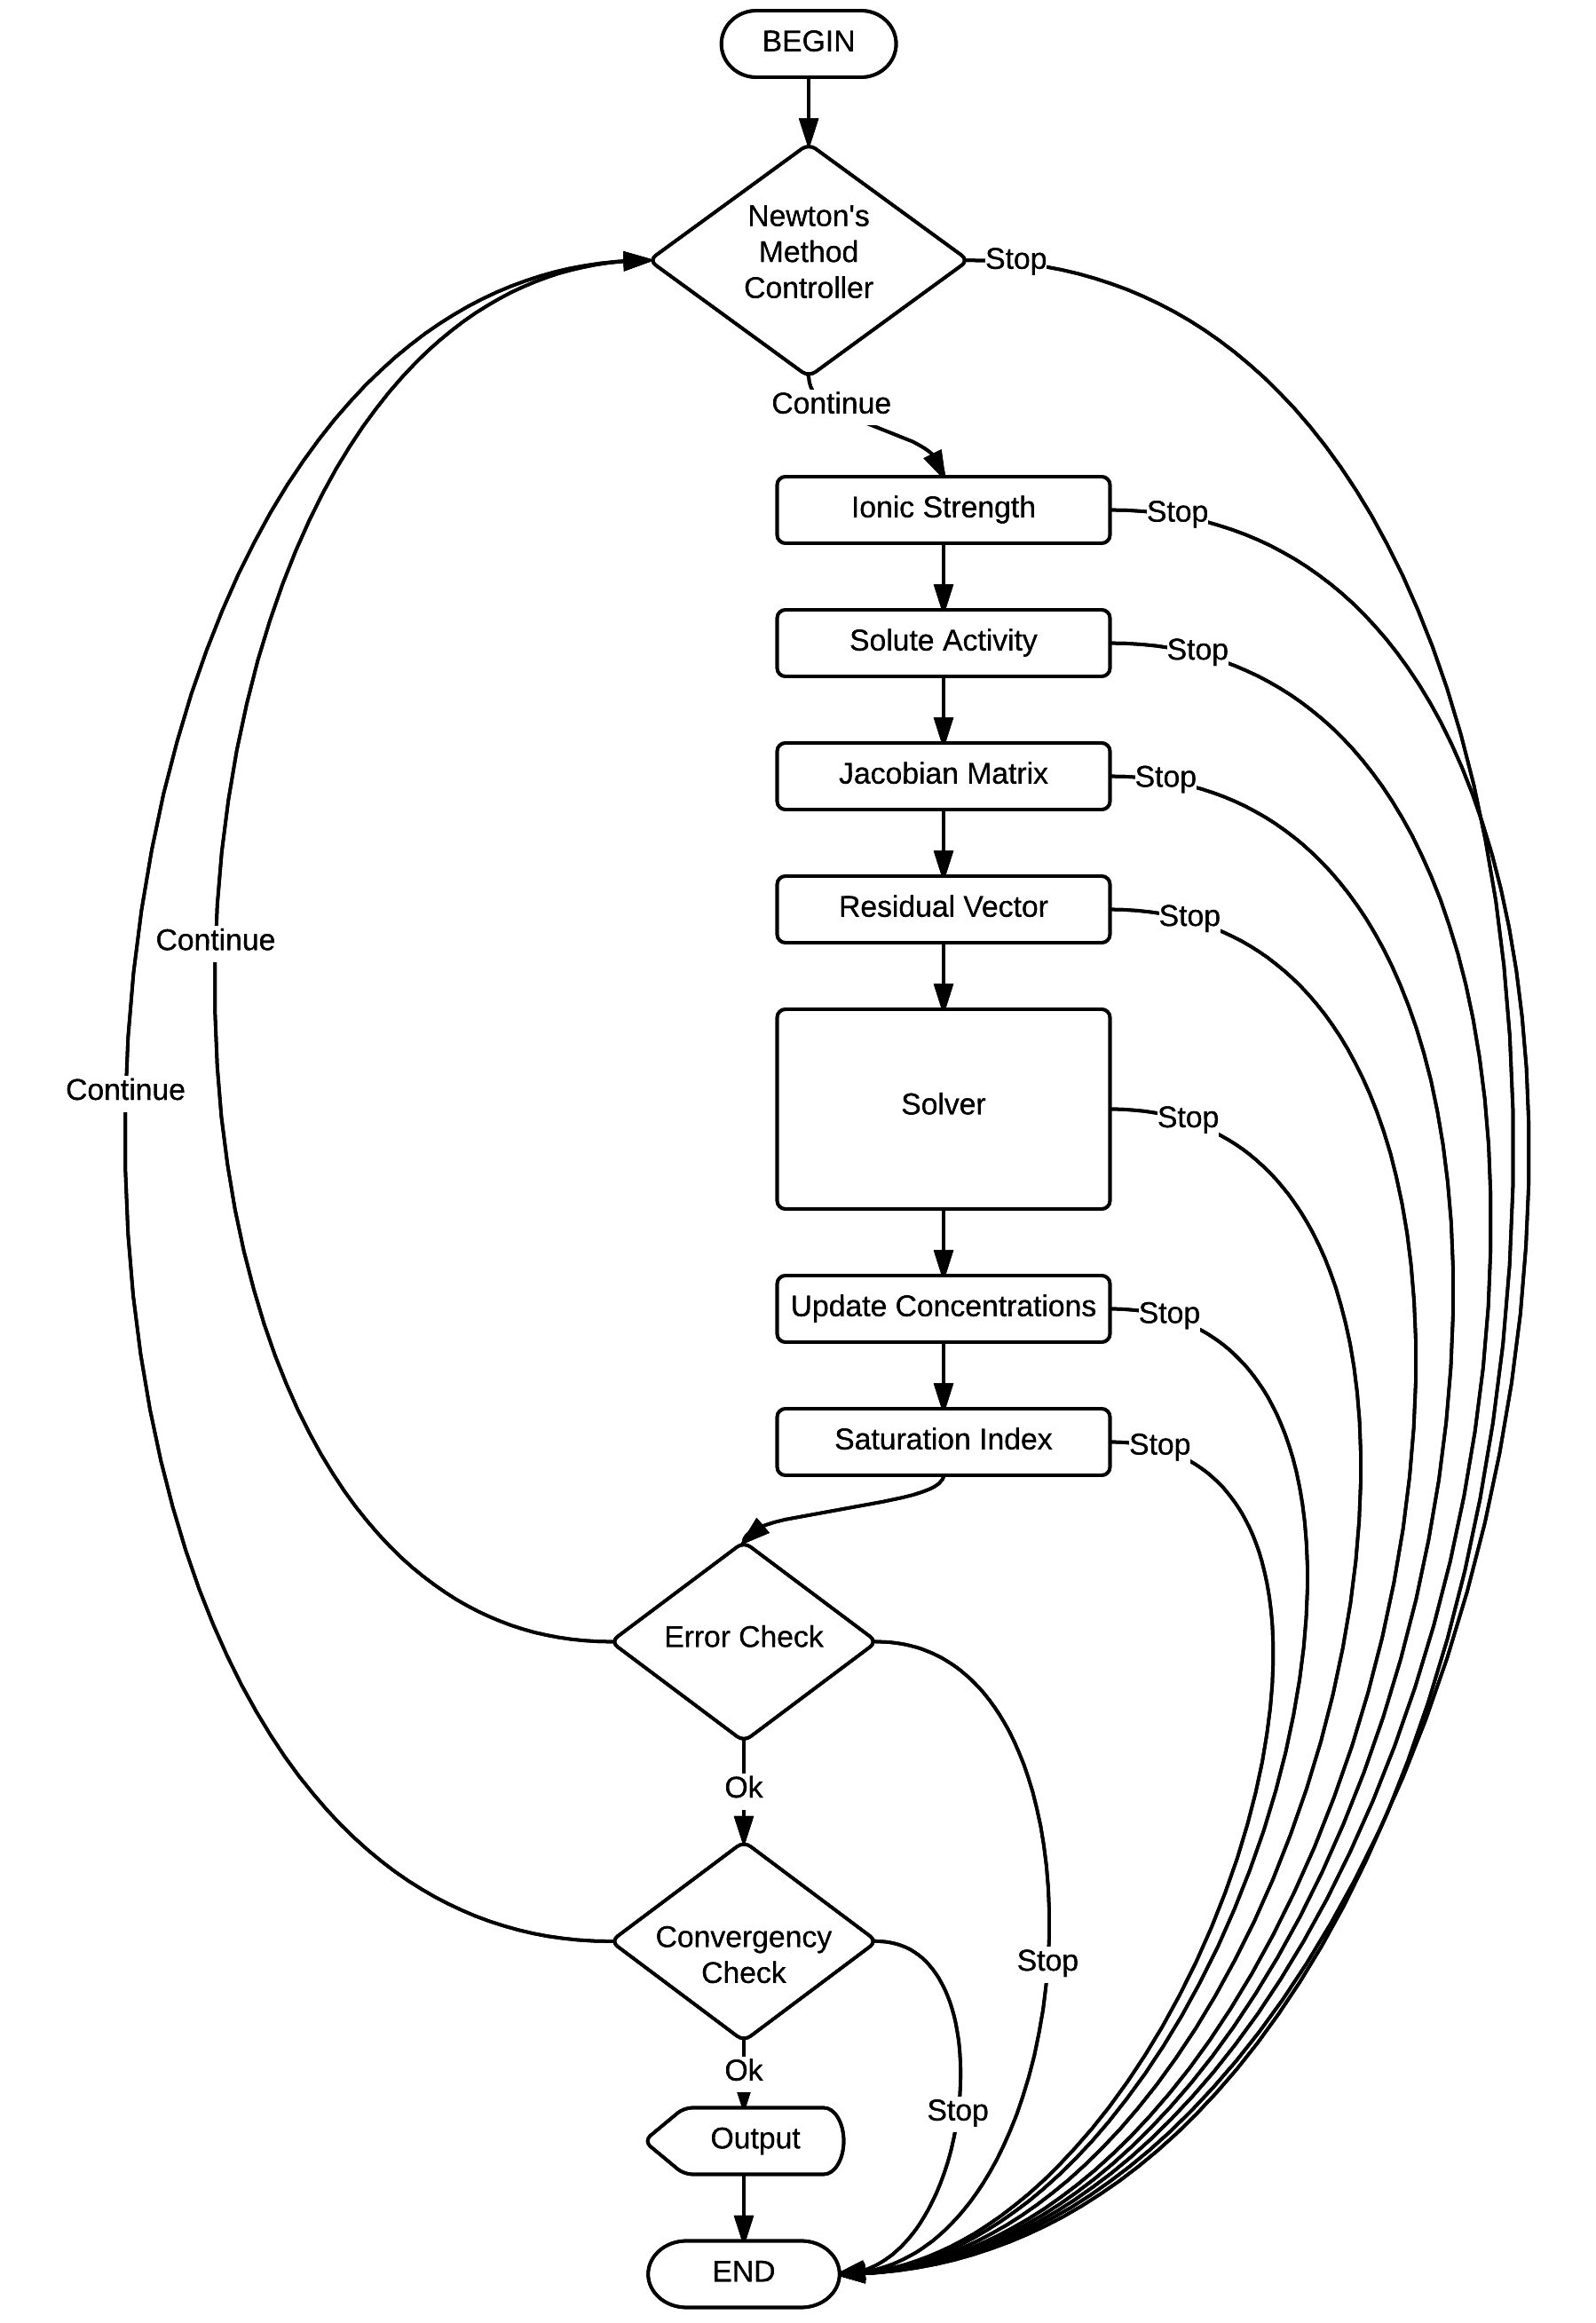
\includegraphics[width=100mm]{figures/Shpeck_algo_newton.png}
\caption{Algorithm of the Newton's Method Solver}
\label{fig:Shpeck-algo-newton}
\end{figure}
\subsection{Complexity of the algorithm}
The Gauss-Newton's method has a complexity O($n^3$) per iteration with a quadratic convergence.

%(http://ranger.uta.edu/~huber/cse4345/Notes/Nonlinear_Equations.pdf)
%(http://ranger.uta.edu/~huber/cse4345/Notes/Equations.pdf)
%(compared to http://en.citizendium.org/wiki/Newton%27s_method#Computational_complexity)


\section{Graphical User Interface}
Due to the enormous amount of options connected to the nature of geochemical modeling, the development of a GUI is a challenge itself. It is necessary to develop a software that is intuitive and user-friendly and has an accurate and efficient approach to all of the options available in nature and the system. The development of the GUI introduces several stages of processes related to it:
\begin{itemize}
	\item Planning : This moment is where the developer needs to think a way to contemplate all the options from the core of the program and make them easily, intuitive and friendly to the final user. The planning is an essential process and must be correct. All the content, features, details of the software need to be strictly defined and organized in order not to break anything afterwards nor forget it (which will result in a not used software). A slight path divides something really useful from something not useful at all - assumptions and the challenge of the developer to think as a user is sometimes tough because many of the developers are not the final user for its applications. Is important also to find out what others have done or are doing - during the study of others software their GUI were analyzed carefully.
	\item Building : All the planning done for needs to be implemented and the main features of the software are important to be well defined at this point. To build the tool \emph{Qt} - already presented above - was chosen due to its many advantages as easy to customize; no coding; templates; simple drag and drop \emph{GUI}  builder; secure and reliable;
	\item Ensuring Usability : The challenge in the field of Human-Computer Interaction (HCI) investigates way people use computers is huge. Techniques and tools are used to find some relevant standards, and some measurements are available. Just to name a few, tests with real users; evaluation by experts; gathering user feedback; Usage logging;
\end{itemize}


\subsection{\emph{SHPECK}'s GUI }
Among geochemical modelling software, the GUI was either not or poorly implemented. We see\emph{SHPECK} as geochemical speciation modelling software with a potential to broaden its influence. The \emph{GUI} enables the user to focus on essential duties and not struggle with the mental power wasted on things that do not matter when modelling a geochemical environment. We think of the GUI with a bright idea that the less skill it requires, the better it is.
\emph{SHPECK}'s GUI works based on tabs, each tab is responsible for viewing an specific point of the software. We present them in details bellow:
\begin{itemize}
\item Configurations tab: Allows users to view and manipulate basic system settings and controls such as temperature, activity coefficient calculation method, the number of iterations, solver options, maximal error and convergence criteria. It is presented in ~\ref{fig:config}.
\item Compounds in the water tab: Allows users to create and edit the composition of the water that will be used in the geochemical speciation model. It has  all the species available from the database and its concentration. The species in the tab that have concentration different than zero compose the water. This tab is presented in ~\ref{fig:water}.
\item Results tab: Allows the user to see relevant input information and the outputs of the geochemical speciation model such temperature, ionic strength, pH of the solution, final concentration for the species, saturation indexes, etc. It is presented in ~\ref{fig:output}
\end{itemize}


\begin{figure}[ht!]
\centering
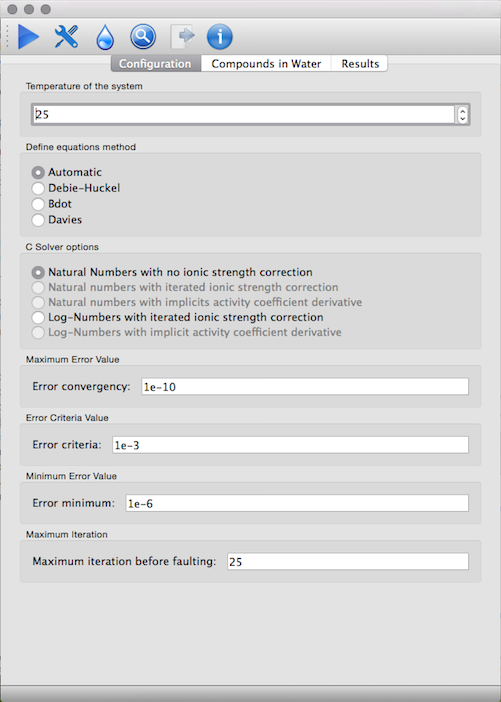
\includegraphics[width=100mm]{figures/shpeck-configtab.png}
\caption{Configuration tab}
\label{fig:config}
\end{figure}

\begin{figure}[ht!]
\centering
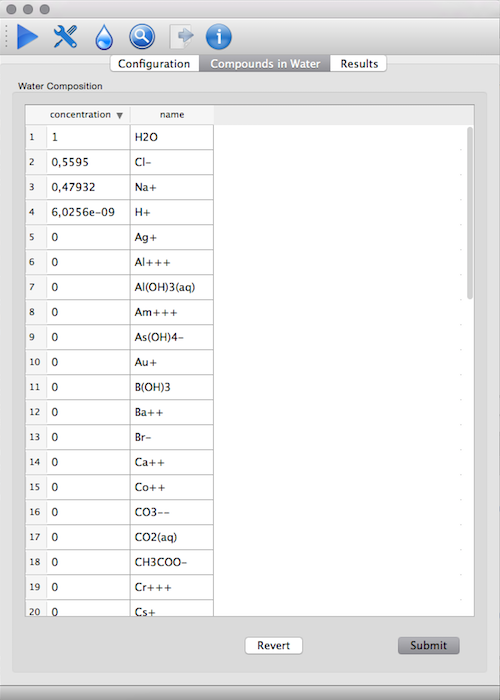
\includegraphics[width=100mm]{figures/shpeck-watertab.png}
\caption{Water composition tab}
\label{fig:water}
\end{figure}

\begin{figure}[ht!]
\centering
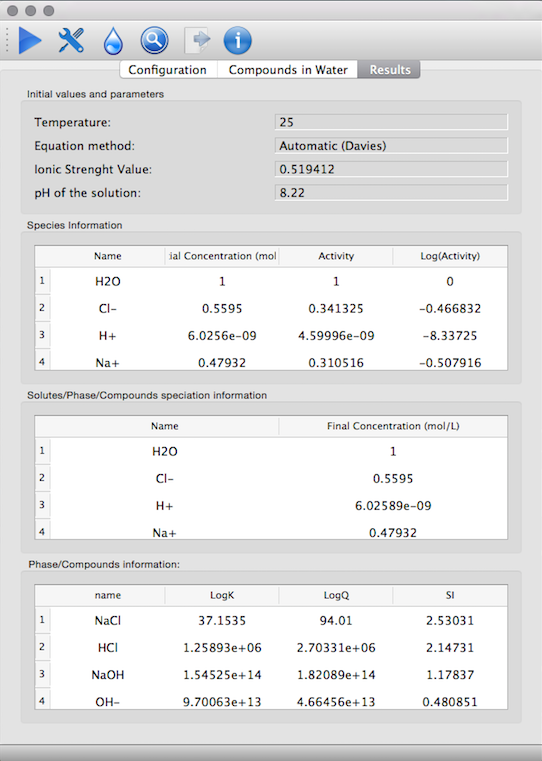
\includegraphics[width=100mm]{figures/shpeck-resultstab.png}
\caption{Results tab}
\label{fig:output}
\end{figure}

\section{Database}
As can be seen in this chapter, the algorithm of \emph{SHPECK} is not trivial and requires many interactions between many different entities. The database is responsible for providing all the data that will flow through and works as the \emph{seed} provider. Chapter ~\ref{chapter:review} makes clear that using a flat file database is something harmful to the software. Potential issues of using flat file databases are duplication of the information; non-unique records; hard to update; inherently inefficient; harder to change data format; poor at complex queries; no security;
In \emph{SHPECK}, we use a relational database, which is a model of a database that prevents all the problems faced in flat file database previously discussed and enable to take full advantage of the information on it. Relational databases work based on a \emph{query}, which is an information request from the database. Besides that, there are three important advantages:
\begin{itemize}
\item A relational database has the advantage of not necessarily be in the memory of the computer - often these databases are larger than the computer's memory. What happens is that the software fetches the information on-the-go. 
\item Complex queries enable the versatility and efficiency when fetching relevant information from the database. Instead of scanning the whole flat file, the query can pre-define the categories of information - even from multiple tables - which will be sought. Also important to mention, a query can be composed and concatenated on runtime execution - meaning that \emph{SHPECK} only fetches from the database information relevant to the specific simulation that is being executed (species, compounds, reactions, etc.). Complex queries and concatenation of queries result in a faster and more efficient use of the available resources.
\end{itemize}

Instead of being something to worry about, the database is one of the most critical and significant infrastructure parts of our software. The database architecture was defined after studying the algorithm and determining what would be the structure and the information needed - it is presented in details in figure ~\ref{fig:ERDiagram}. We developed a relational database that embrace all the important data already in use from other software but with a newer approach and structured in tables - naturally some changes in the structure were necessary in order to compact, organize, structure and make it easier to use.

\begin{figure}[ht!]
\centering
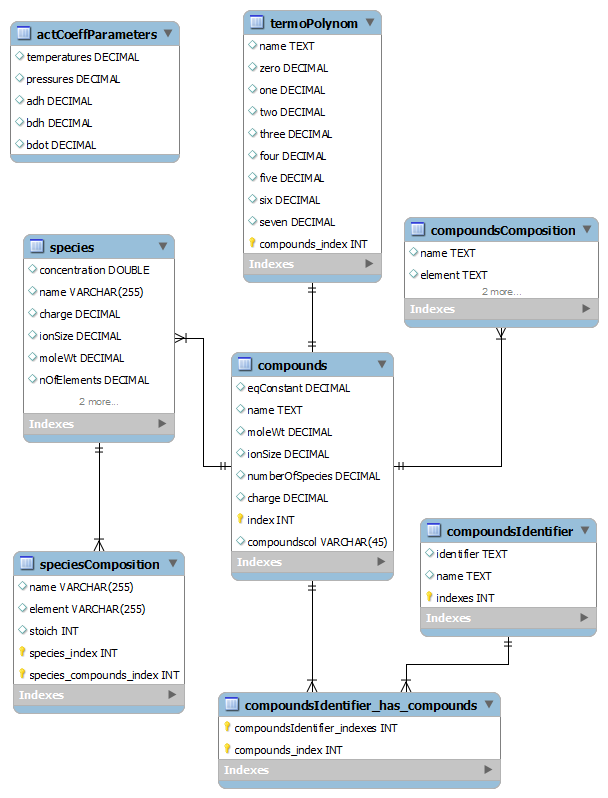
\includegraphics[width=100mm]{figures/ER_diagram.png}
\caption{ER Diagram of the database}
\label{fig:ERDiagram}
\end{figure}

\subsection{Database Technologies}
We use the SQLite database \cite{SQLite}, which is a software library that implements a self-contained, transactional \emph{SQL} database engine, open source and currently is the most widely deployed \emph{SQL} database engine in the world. Some of its advantages are explained bellow:
\begin{itemize}
\item Zero-Configuration: \emph{SQLite} does not need to be installed before it is used, there is no setup procedure;
\item Serverless: The process that wants to acess the database reads and writes directly from the database files on disk. There is no intermediary server process (nor interprocess communication using \emph{TCP/IP});
\item Single Database File: An \emph{SQLite} database is a single file located in the directory hierarchy. \emph{SQLite} database can be easily copied onto a USB memory stick or emailed for sharing;
\item Stable Cross-Platform Database File: A database file written on one machine can be copied and used on a different machine with a different architecture. Furthermore, \emph{SQLite} is backwards compatible (newer versions can read and write older database files);
\end{itemize}

\subsection{\emph{LLNL} thermodynamic dataset parser}
Once we defined what would be the structure and the technology of our database, we need to find the information to populate it - the information that would  feed \emph{SHPECK}. We create a parser for the flat file database that extracted the information and arranged it following our structure. 
The parser was carefully generated in order not to misunderstand any structure nor miss a delimiter - this task was extremely time-consuming and proportionally important for the success of \emph{SHPECK}.

\newpage

\section{Summary}
\begin{itemize}
\item Architecture: \emph{SHPECK} follows the architectural pattern called \emph{MVC}; It's benefits are the complete separation of responsibilities and concerns among the parts of the software; there is no mixing of codes between them. Another advantage that worth mentioning is the flexibility for the software to grow and develop itself. Figure ~\ref{fig:shpeck-architecture} displays the \emph{MVC} pattern existing in \emph{SHPECK}.
\item Governing Equations: \emph{SHPECK} is a geochemical speciation modelling software that drives the behaviour of the aqueous system based on a set of mass-action equations combined with equilibrium constraints. A mass-action equation is described in equation  ~\ref{eq:massaction} and reinforced here:

\begin{equation}
K_j =  \prod\limits_{i=1}^N  a_i^{v_{ij}} \hspace{35pt}    (j = 1, ... , M)
\end{equation}

where $K_j$ denotes the equilibrium constant of the \emph{j-th} reaction; $a$ denotes the activity of the \emph{i-th} chemical species.

\item Numerical Method: \emph{SHPECK} applies the \emph{Gauss-Newton's} method to solve the nonlinear system of equations. The concept of the method is described in equation ~\ref{eq:gaussNewtonMethodEq1} and reinforced here:

\begin{equation}
F(x+1) = F(x) - J^{-1} * R
\end{equation}

Where $F$ is function's result for the applied $x$, $J^{-1}$ is the inverse of the Jacobian matrix, and $R$ is the residual matrix. The quadratic rate of convergence of this method compensate the expensive calculation inherent to it.

\item Graphical User Interface: The \emph{GUI} mission is to enable the user to use fully the potential \emph{SHPECK} has to offer. It is intuitive and user-friendly to allow the user to focus on essential duties that are imperative to model a geochemical environment. We use the popular approach of \emph{tab} panels, which are separated according the purpose of it: configurations and settings, water composition and results visualization.
\item Database: A geochemical modelling software is severely dependent on the information inside it. \emph{SHPECK} structure all of its data in a \emph{SQLite} relational database, unique among the commercial software available. \emph{SHPECK}'s database is composed by the information about elements, species, compounds, reactions and thermodynamic constants from the \emph{LLNL} thermodynamic dataset. A parser for \emph{LLNL} flat file database was created to fetch this information.
\end{itemize}